%%% Local Variables: 
%%% coding: utf-8
%%% mode: latex
%%% TeX-engine: xetex
%%% End: 

\documentclass[hide notes,intlimits]{beamer}

\mode<presentation>
{
  \usetheme[footline]{PISMshade}
  \setbeamercovered{transparent}
}

% load packages
\usepackage{media9}
\usepackage[english]{babel}
\usepackage[multidot]{grffile}

\usepackage{tikz}
\usetikzlibrary{shapes,arrows}
\usetikzlibrary{shadows}

\definecolor{dark red}{HTML}{E41A1C}
\definecolor{dark green}{HTML}{4DAF4A}
\definecolor{dark violet}{HTML}{984EA3}
\definecolor{dark blue}{HTML}{084594}
\definecolor{dark orange}{HTML}{FF7F00}
\definecolor{light blue}{HTML}{377EB8}
\definecolor{light red}{HTML}{FB9A99}
\definecolor{light violet}{HTML}{CAB2D6}

\setbeamercolor{boxed}{fg=black,bg=light blue!25}
\graphicspath{{../figures_2018_08/}{../figures/}}

\newenvironment{transbox}[1][]{%
\begin{tikzpicture}
\node[drop shadow,rounded corners,text width=.9\textwidth,fill=white, fill opacity=#1,text opacity=1] \bgroup
}{
\egroup;\end{tikzpicture}} 

\newenvironment{transbox-tight}{%
\begin{tikzpicture}
\node[drop shadow,rounded corners,fill=uaf yellow, fill opacity=0.75,text opacity=1] \bgroup
}{
\egroup;\end{tikzpicture}} 

\newcommand{\jl}{[\![}
\newcommand{\jr}{]\!\hskip 0.003cm ]}
\newcommand{\bpsi}{\boldsymbol{\psi}}
\newcommand{\bPsi}{\boldsymbol{\Psi}}
\newcommand{\bphi}{\boldsymbol{\phi}}
\newcommand{\bPhi}{\boldsymbol{\Phi}}
\newcommand{\bn}{\mathbf{n}}
\newcommand{\bq}{\mathbf{q}}
\newcommand{\bv}{\mathbf{v}}
\newcommand{\D}{\,\mathrm{d}}
\newcommand{\Tsnow}{T_{\text{snow}}}
\newcommand{\Hatm}{H_{\text l}^{\text{atm}}}

\newcommand{\mathtext}[1]{\mathsf{#1}}

% title page
\title[Ice sheet modeling] % (optional, use only with long paper titles)
{The Greenland Ice Sheet ---\\ Will it stay or will it go?}

\author[Aschwanden] % (optional, use only with lots of authors)
{\textbf{Andy Aschwanden}, M. Fahnestock, M. Truffer, D. Brinkerhoff, R. Hock, C. Khroulev, R. Mottram, A. Khan}
\institute{Geophysical Institute, University of Alaska Fairbanks}

% - Give the names in the same order as the appear in the paper.
% - Use the \inst{?} command only if the authors have different
%   affiliation.

% - Use the \inst command only if there are several affiliations.
% - Keep it simple, no one is interested in your street address.

\titlegraphic{\vskip-1.cm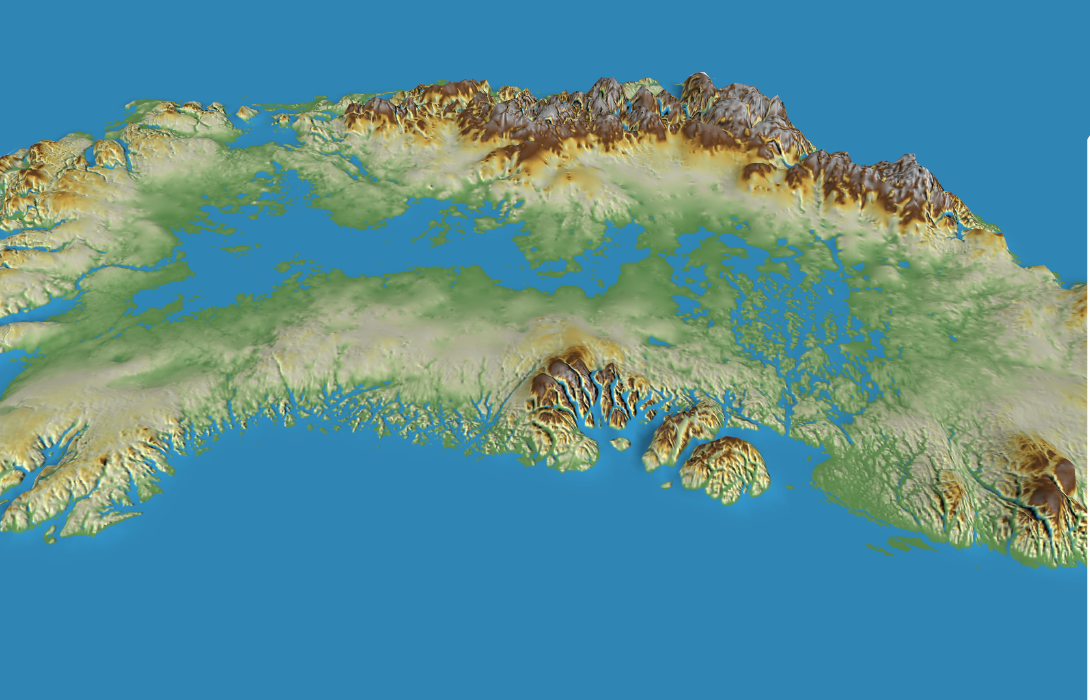
\includegraphics[height=3.5cm]{gris-green-collage-clean}}

\date{}


\subject{The Greenland Ice Sheet}

\begin{document}


\setbeamertemplate{background canvas}
  {
     \tikz{\node[inner sep=0pt,opacity=1.0] {\includegraphics[width=\paperwidth]{uaf_beamer_shade_bg}};}
} 

% insert titlepage
\begin{frame}
  \titlepage
  \note[item]{Collaboration between most glaciology faculty at UAF}
  \note[item]{Mark F., Martin T., Regine H., and my former student Doug B.}
\end{frame}


\setbeamertemplate{background canvas}
  {
     \tikz{\node[inner sep=0pt,opacity=1] {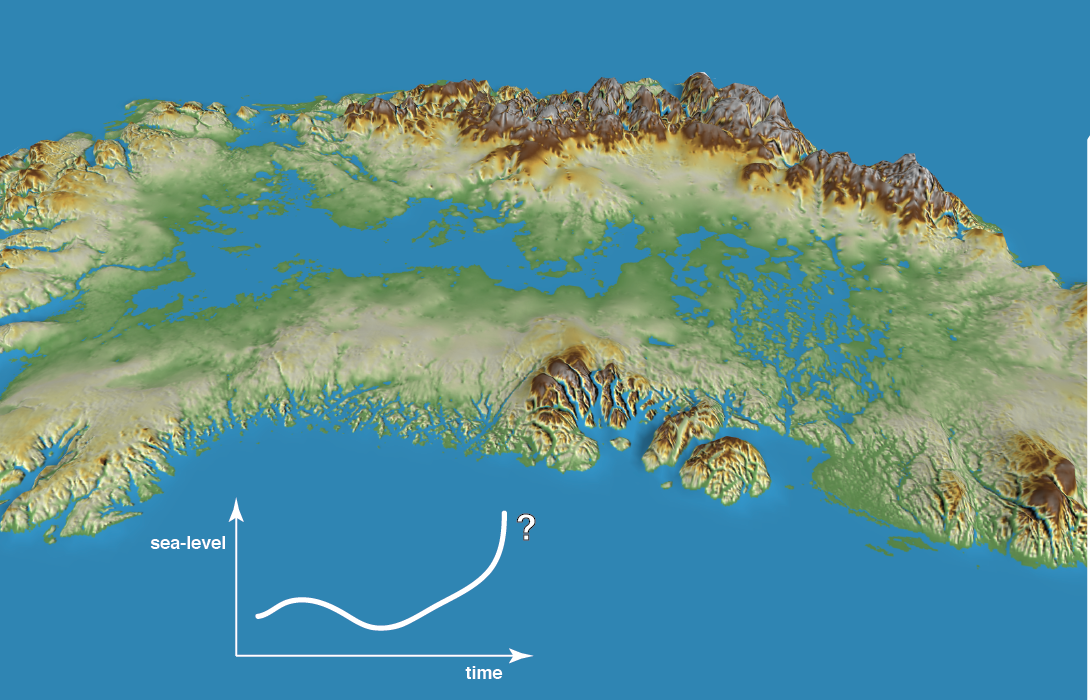
\includegraphics[height=\paperheight,width=\paperwidth]{gris-green-collage-slr}};}
} 

\begin{frame}[plain]
  \note[item]{We know Greenland was nearly ice-free for extended periods during the Pleistocene}
  \note[item]{that's from 2.6 million years ago to 11,700 years ago}
  \note[item]{Maybe Greenland looked somehting like this}
  \note[item]{}
\end{frame}


\setbeamertemplate{background canvas}
{
%
}



\begin{frame}{Observed vs simulated flow speeds (2013 model)}
  \begin{columns}[c]
    \begin{column}{.6\linewidth}
    \begin{figure}
      \includegraphics[width=0.9\textwidth]{gris-obs-exp-old}
      \\ \tiny{adapted from Aschwanden, Fahnestock, Truffer (2016) \textit{Nature Comms.}}
    \end{figure}
    \end{column}
    \begin{column}{.4\linewidth}
      \begin{figure}
        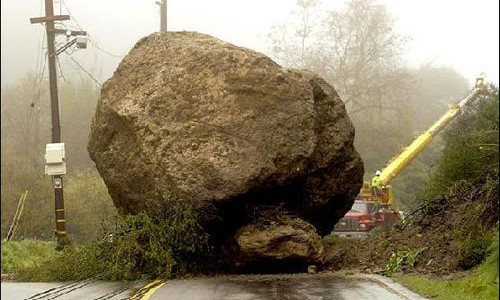
\includegraphics[width=\textwidth]{roadblocks}
      \end{figure}
      \begin{itemize}
      \item can't reproduce the velocity field
      \end{itemize}
    \end{column}
  \end{columns}
  \note[item]{}
\end{frame}


\begin{frame}{Accurate ice thickness does the trick}
  \begin{columns}[c]
    \begin{column}{.6\linewidth}
    \begin{figure}
      \includegraphics[width=0.9\textwidth]{gris-obs-exp-new}
      \\ \tiny{adapted from Aschwanden, Fahnestock, Truffer (2016) \textit{Nature Comms.}}
    \end{figure}
    \end{column}
    \begin{column}{.4\linewidth}
      \begin{figure}
        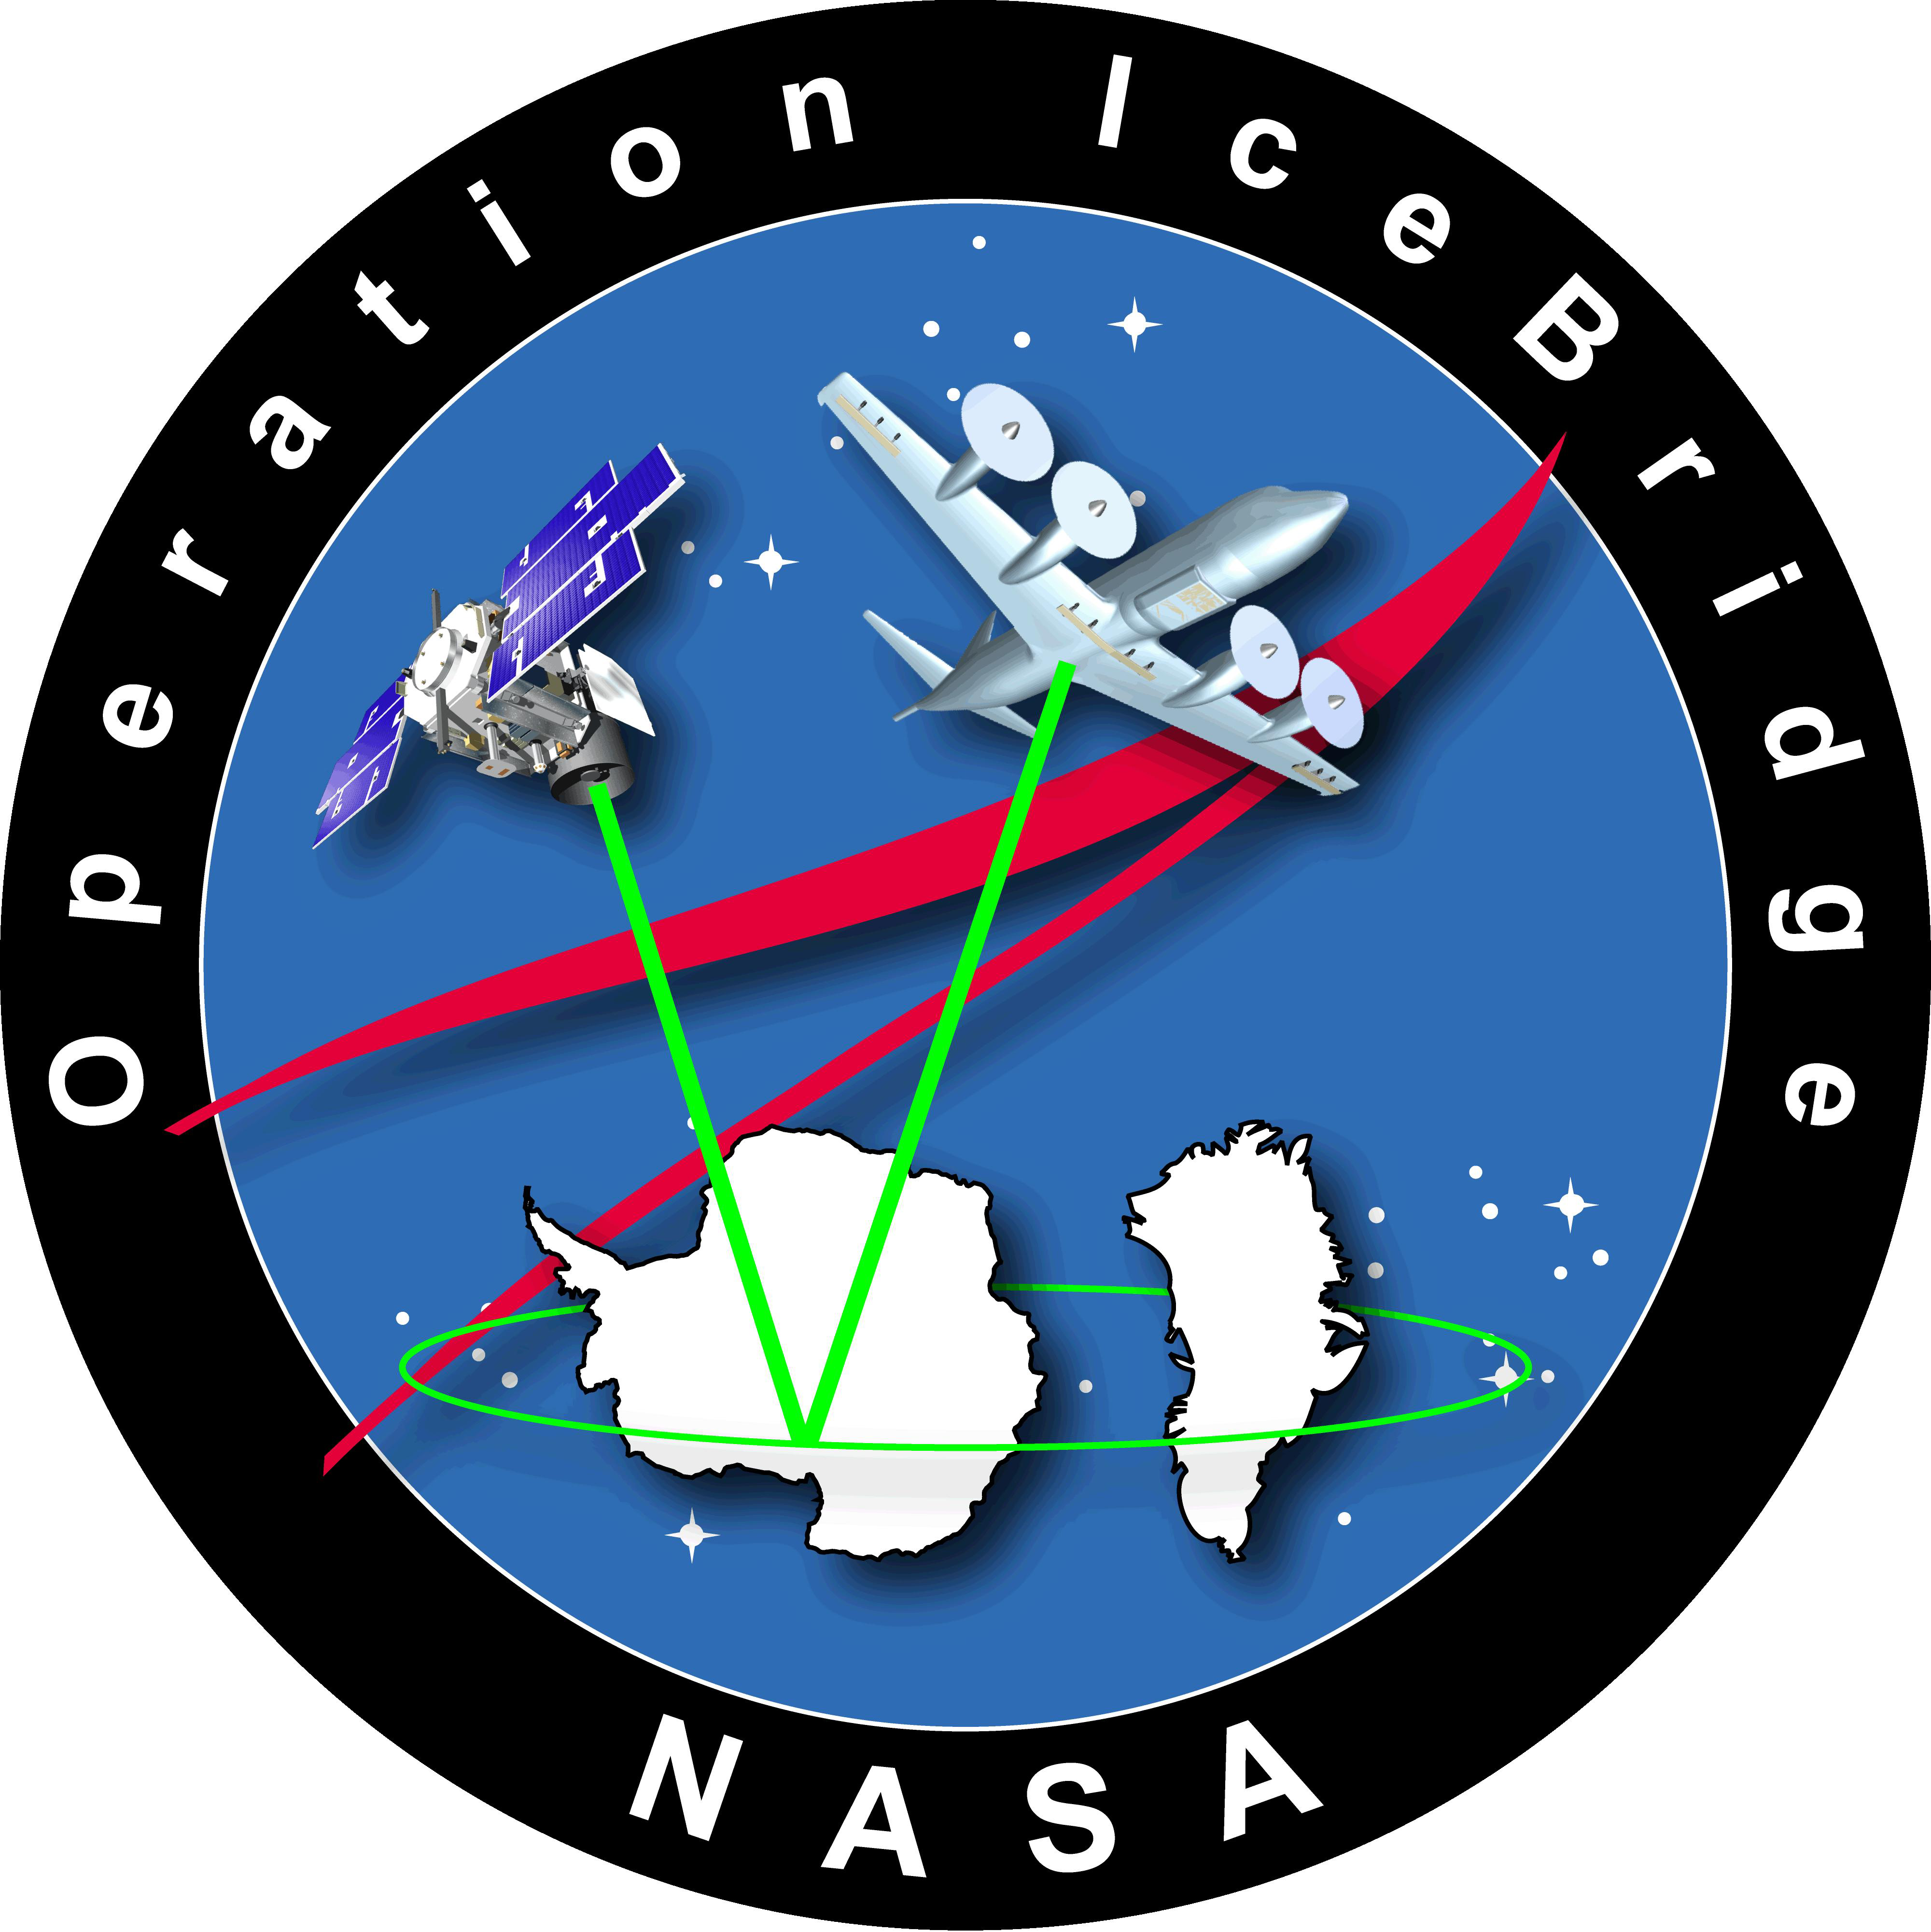
\includegraphics[height=1cm]{oib} \\
        \includegraphics[width=.7\textwidth]{greenland-bed-mcb}
      \\ \tiny{adapted from Morlighem et al.  (2014) \textit{Nature Geosci}}
      \end{figure}
    \end{column}
  \end{columns}
  \note[item]{first time capturing the flow field for the right reason}
  \note[item]{this is quite a break through in ice sheet modeling}
  \note[item]{though not a surprising one}
  \note[item]{it just confirms what students learn in glaciology 100:}
  \note[item]{ice flows downhill}
\end{frame}

\begin{frame}{A new outlet glacier resolving assessment}
  \begin{figure}
    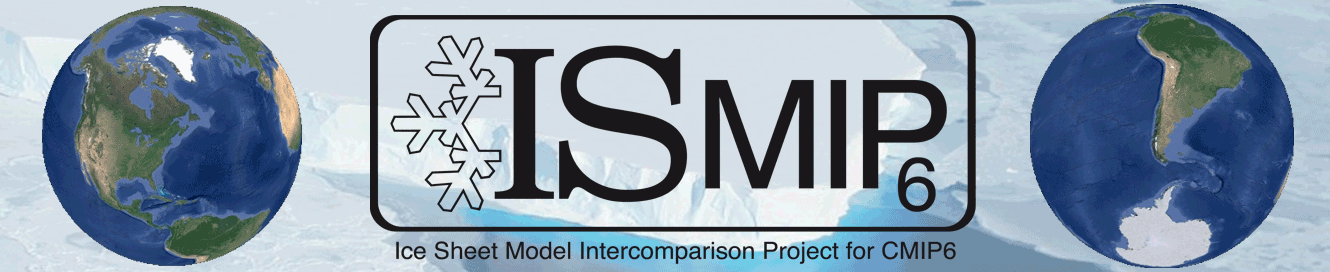
\includegraphics[width=4cm]{ismip6_logo}
  \end{figure}
  \begin{figure}
    \includegraphics[width=10cm]{gris-pism-setup-2018}
  \end{figure}
  \note[item]{Over the past year, we've assembled the best data sets}
  \note[item]{added new model physics such better calving parameterizations}
  \note[item]{don't look at the figures carefully}
  \note[item]{to bring you the first post-AR5 sea level estimates}
  \note[item]{for the next millennium}
\end{frame}


\begin{frame}
  \frametitle{In a thousand years}
  \begin{figure}
    \includegraphics[width=11cm]{rcp-final-states-speeds}
  \end{figure}
  \note[item]{In a thousand years, Greenland will look different to today}
  \note[item]{Explain uncertainty map}
\end{frame}


\begin{frame}
  \frametitle{Uncertainty Quantification}
    \begin{figure}
    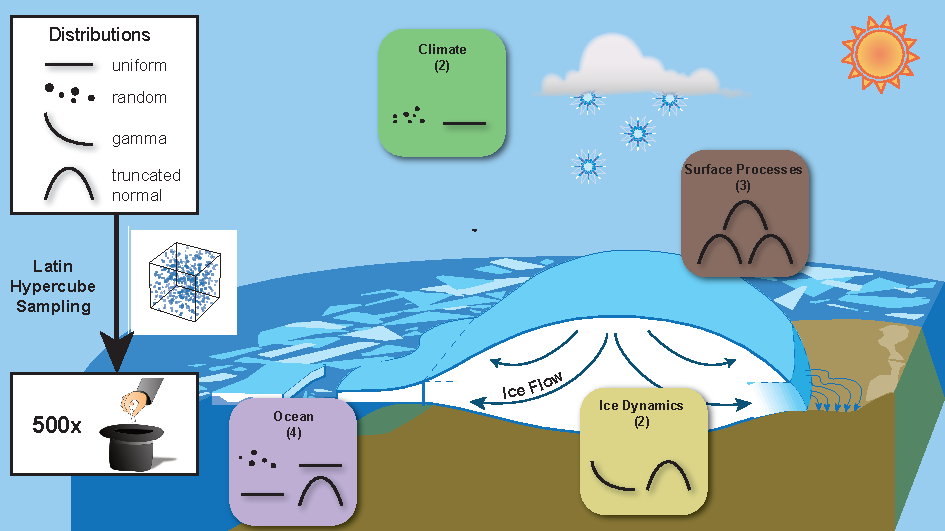
\includegraphics[width=\textwidth]{uncertainty-quantification}
    \end{figure}
\end{frame}

\begin{frame}
  \frametitle{In a thousand years}
  \begin{figure}
    \includegraphics[height=6.5cm]{rcp-final-states-extend}
  \caption{Likelihood of a pixel being ice covered. Likelihoods less than 16 percent are masked.}
  \end{figure}
  \note[item]{In a thousand years, Greenland will look different to today}
  \note[item]{Explain uncertainty map}
\end{frame}

\begin{frame}
  \frametitle{Evolution over the next millennium}
  \begin{figure}
    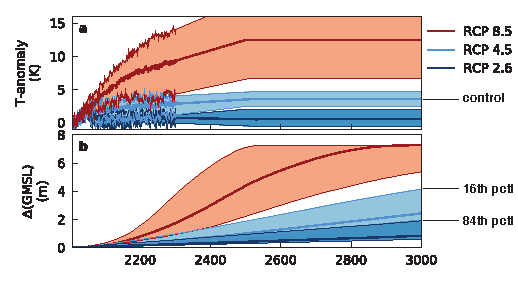
\includegraphics[width=0.95\textwidth]{gris-les}
  \end{figure}
  \begin{columns}[c]
    \begin{column}{.6\linewidth}
  \small{
    For RCP 8.5:
  \begin{itemize}
  \item 67\% of the ensemble members lose $>$90\%
  \item 58\% lose $>$99\% of initial ice volume.
  \end{itemize}
  }
    \end{column}
    \begin{column}{.4\linewidth}
      \small{
        Question:
      \begin{itemize}
      \item what contributes to the uncertainty
      \end{itemize}
      }
    \end{column}
  \end{columns}
\end{frame}


\begin{frame}{Uncertainty attribution using Sobel Indices}
  \begin{figure}
    \includegraphics<1>[width=\textwidth]{sobel_ts}
  \end{figure}
\end{frame}

\begin{frame}[plain]
  \begin{figure}
  \includemedia[
  width=12cm,
  activate=pageopen,
  addresource=nw-g600m_rcp_45-hd1920.mp4,
  flashvars={src=nw-g600m_rcp_45-hd1920.mp4}
  ]
  {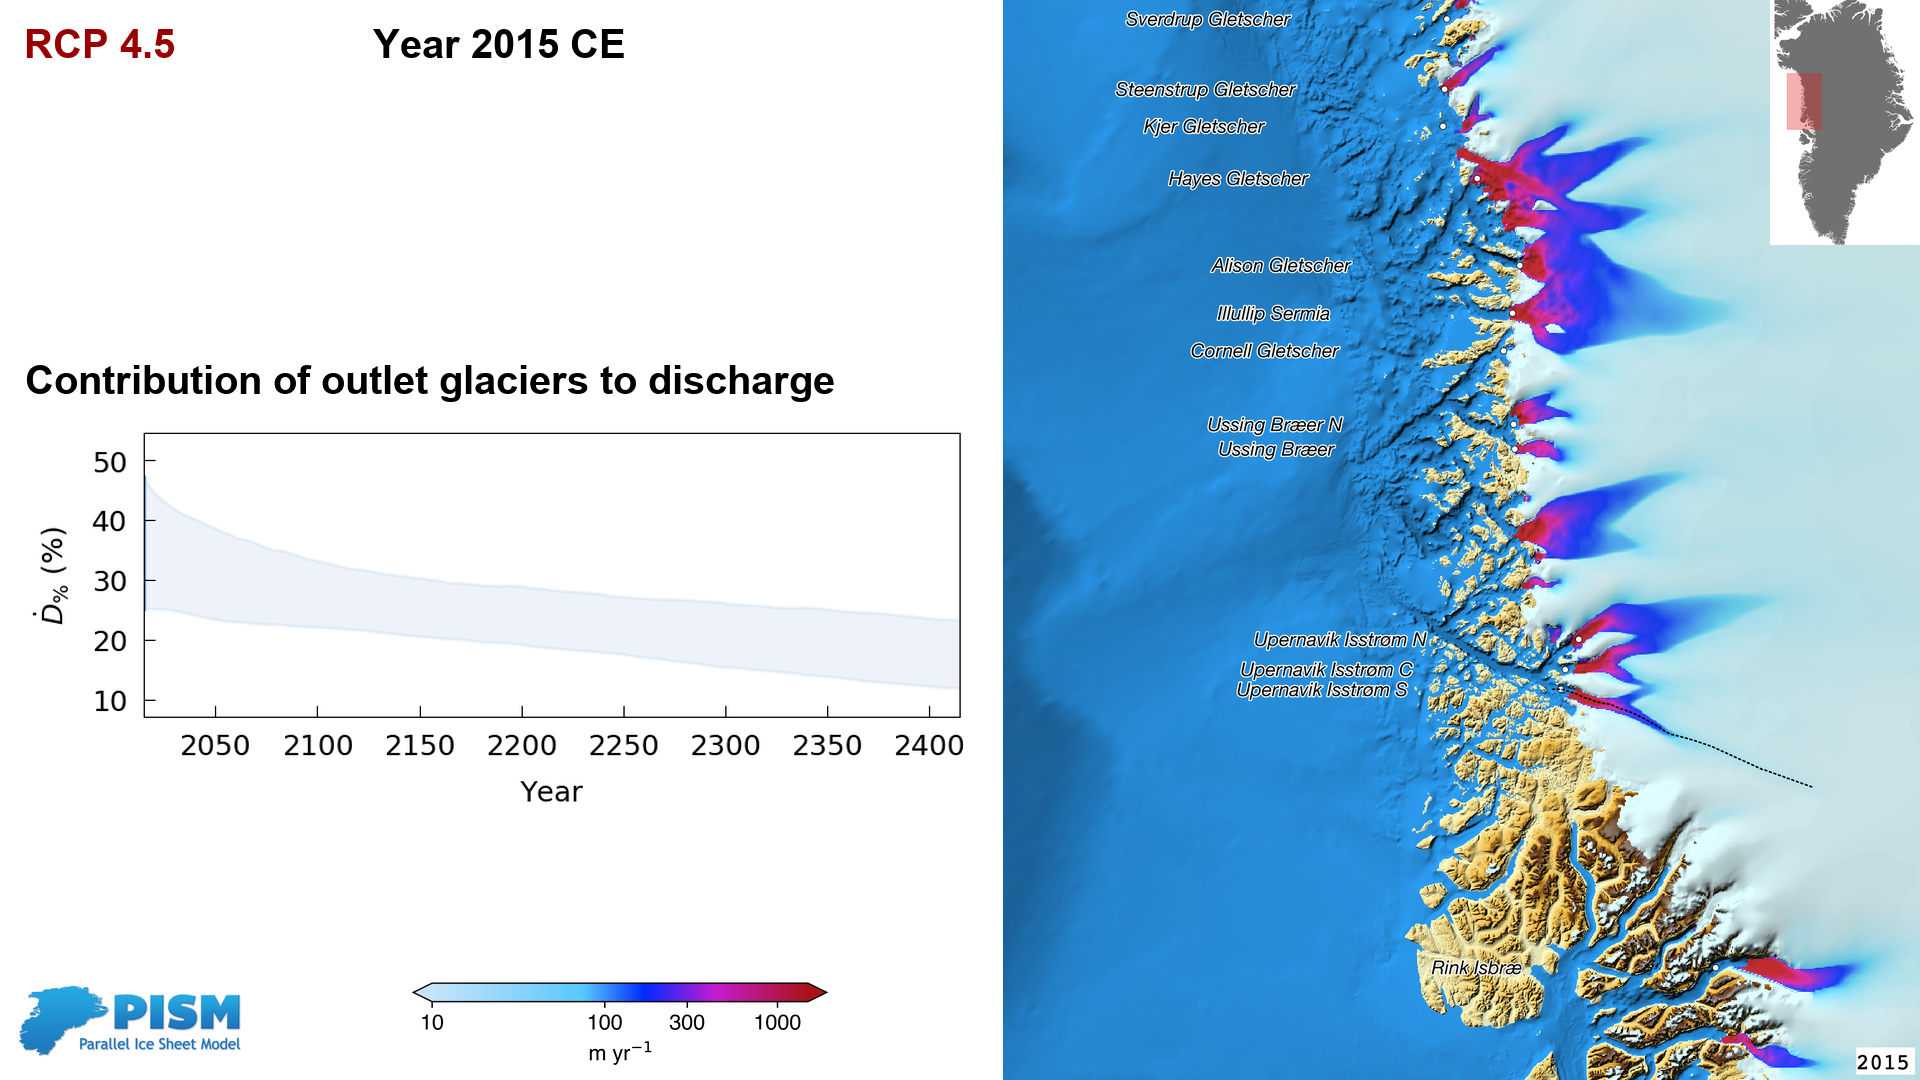
\includegraphics[width=12cm]{nw_g600m_rcp45_0000}}{StrobeMediaPlayback.swf}
\end{figure}
\end{frame}

\begin{frame}[plain]
  \begin{figure}
  \includemedia[
  width=12cm,
  activate=pageopen,
  addresource=upernavik-g600m_rcp_45-hd1920.mp4 ,
  flashvars={src=upernavik-g600m_rcp_45-hd1920.mp4
  }
  ]
  {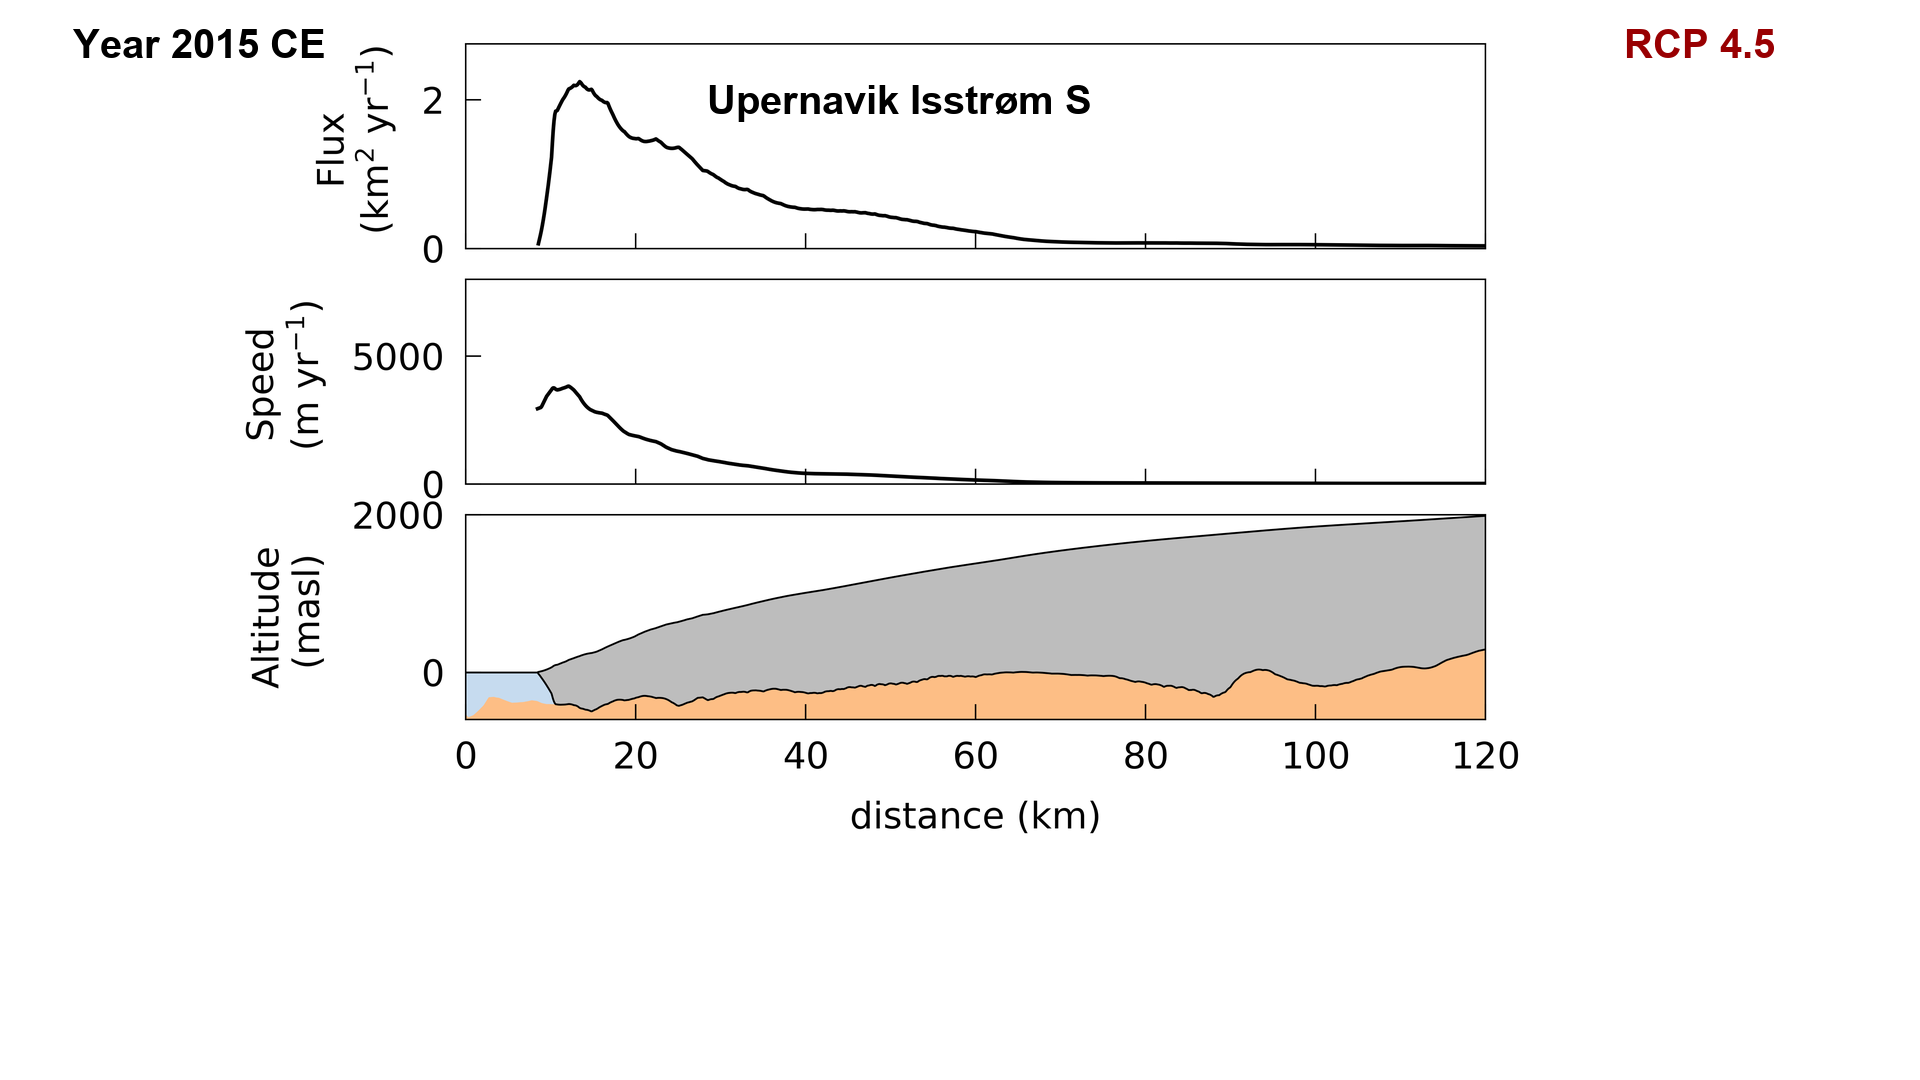
\includegraphics[width=12cm]{upernavik_g600m_rcp45_0000}}{StrobeMediaPlayback.swf}
\end{figure}
\end{frame}

\begin{frame}{Postdoc available, aaschwanden@alaska.edu}
  \begin{figure}
  \includemedia[
  width=7cm,
  activate=pageopen,
  addresource=gris-g900m_rcps-hd1920.mp4,
  flashvars={src=gris-g900m_rcps-hd1920.mp4
  }
  ]
  {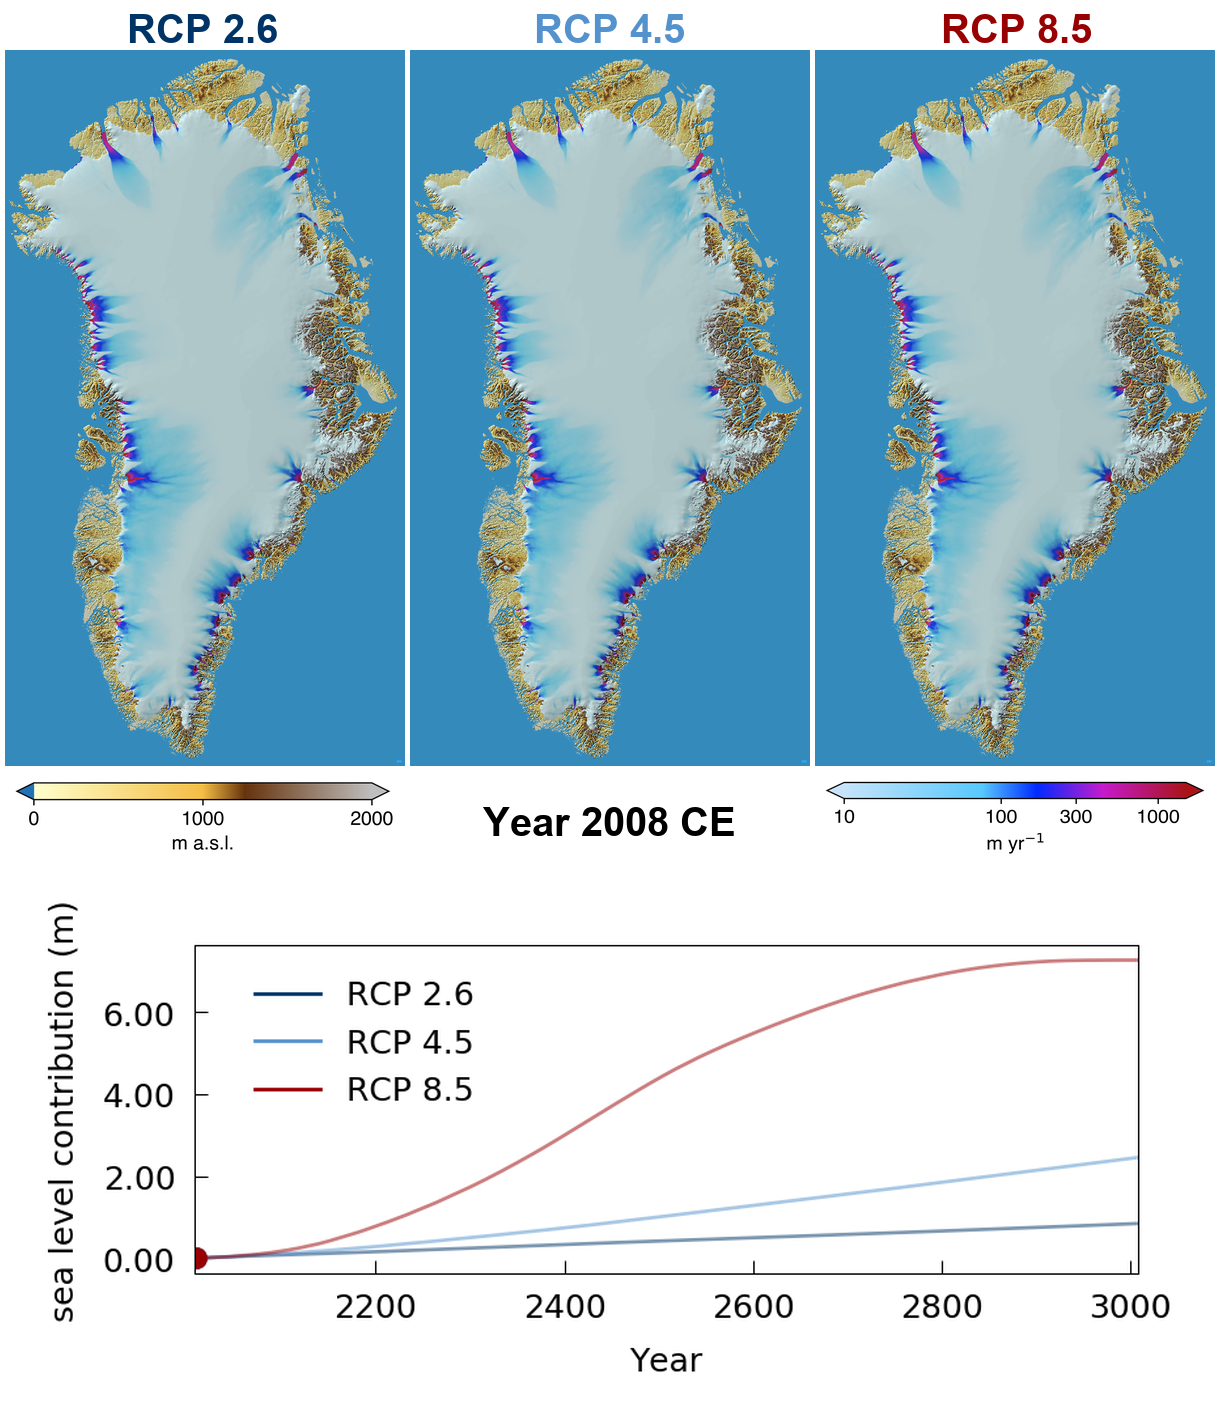
\includegraphics[width=7cm]{gris_g900m_rcps_0000}}{StrobeMediaPlayback.swf}
\end{figure}
\end{frame}

\end{document}